\documentclass[sigplan,screen]{acmart}

\copyrightyear{2026}
\acmYear{2026}
\setcopyright{cc}
\setcctype{by}
\acmConference[ECOOP-C '26]{ECOOP-Companion}{June 29--30, 2026}{Brussels, Belgium}
\acmBooktitle{ECOOP-Companion (ECOOP-C '26), June 29--30, 2026, Brussels, Belgium}
\acmDOI{10.1145/3849733.3849786}
\acmISBN{979-8-4007-2540-1/2026/06}
\graphicspath{{assets/}}

\usepackage{listings}
\lstset{
  basicstyle=\small\ttfamily,
  columns=flexible,
  keepspaces=true,
  xleftmargin=1em,
  aboveskip=0.6\baselineskip,
  belowskip=0.6\baselineskip,
}
\lstdefinelanguage{MLsem}{
  morekeywords={val,let,if,then,else,is},
  morecomment=[n]{(*}{*)},
  morestring=[b]",
}

% Discourage (but allow) a column break right after displays, code
% listings and lists, so they stay with the text that follows.
% listings ends each listing with \penalty-50, which invites a break.
\usepackage{etoolbox}
\makeatletter
\patchcmd{\lst@DeInit}{\penalty-50}{\penalty5000}{}
  {\errmessage{Could not patch the penalty after listings}}
\@endparpenalty=5000
% Never split a list between its items.
\@itempenalty=10000
\makeatother
\postdisplaypenalty=5000

\newcommand{\ttt}[1]{\texttt{#1}}
\newcommand{\interp}[1]{\llbracket #1 \rrbracket}
\usepackage{stmaryrd}

\begin{document}

\title{Interactive Typing Toolkit: The Types You Want}

\author{Oliver Tu\v{s}la}
\orcid{0009-0003-5459-5820}
\affiliation{%
  \institution{Czech Technical University in Prague}
  \city{Prague}
  \country{Czech Republic}}
\email{tuslaoli@fit.cvut.cz}

\author{Micka\"el Laurent}
\orcid{0000-0003-1590-2392}
\affiliation{%
  \institution{Charles University}
  \city{Prague}
  \country{Czech Republic}}
\email{mickael.laurent@matfyz.cuni.cz}

\author{Pierre Donat-Bouillud}
\orcid{0000-0003-4455-1130}
\affiliation{%
  \institution{Czech Technical University in Prague}
  \city{Prague}
  \country{Czech Republic}}
\email{pierre.donat.bouillud@fit.cvut.cz}

\begin{abstract}
  Set-theoretic type systems infer precise polymorphic
  types for unannotated functions in dynamic languages, capturing
  overloaded behaviour through intersections, unions, and negations
  of types. The price of this precision is readability: inferred
  signatures are often far more verbose than the type a programmer
  would write by hand.  Worse, an overly precise signature
  propagates through inference into every definition that uses it,
  so simplifying one signature can yield more straightforward types
  across the entire codebase.  We present an interactive typing
  toolkit ---
  a VS~Code extension backed by an LSP server on top of the MLsem
  typing library --- that lets the programmer reshape an inferred
  type through simple, semantically justified operations such as
  \emph{instantiation} of type variables and \emph{merging} of
  overloads, exploring the spectrum of correct types for a function
  and choosing where on the precision--readability scale to stop.
  Readability is not the only concern: a narrower contract than the
  code happens to admit can also capture intent.  We outline
  the toolkit's design and our plans to apply it to the R language.
\end{abstract}


\keywords{set-theoretic types, semantic subtyping, type inference,
  dynamic languages, IDE tooling}

\maketitle

\section{The type you get vs.\ the type you want}

Dynamic languages are full of functions whose behaviour is richer
than any simple type suggests: JavaScript's \ttt{||} operator, for
one, is \emph{not} boolean.  \ttt{0 || "x"} evaluates to \ttt{"x"},
and \ttt{\{\} || 1} to \ttt{\{\}}. The operator is
exactly this function~\cite{polymorphic-inference}:

\begin{lstlisting}[morekeywords={function,if,else,return}]
function logical_or(x, y) {
  if (x) { return x; } else { return y; }
}
\end{lstlisting}

The naive type $(\ttt{bool}, \ttt{bool}) \rightarrow \ttt{bool}$
rejects both uses above.  A type system based on set-theoretic types
instead infers a type accounting for all of
them:
\[
  \forall \alpha, \beta.\;
  ((\alpha \wedge \ttt{truthy}, \ttt{any}) \rightarrow \alpha \wedge \ttt{truthy})
  \;\wedge\;
  ((\ttt{falsy}, \beta) \rightarrow \beta)
\]
This type is precise --- but probably not the
type you expected.

We present a VS~Code extension that lets the programmer
\emph{interactively reshape} an inferred set-theoretic type,
choosing for each function where on the precision--readability scale
to stop.

\section{Set-theoretic types}

Our toolkit is built on the MLsem typing
library~\cite{type-inference}, which implements polymorphic type
inference with set-theoretic types and semantic subtyping.  The
guiding intuition is that a type \emph{is} the set of values it
accepts --- its interpretation $\interp{t}$ --- and each type
connective is the matching set operation:
\[
  \interp{\ttt{42}} = \{\ttt{42}\}
  \qquad
  \interp{\ttt{int}} = \{\ldots, 0, 1, \ldots\}
\]
\[
  \interp{t_1 \wedge t_2} = \interp{t_1} \cap \interp{t_2}
  \qquad
  \interp{t_1 \vee t_2} = \interp{t_1} \cup \interp{t_2}
\]
Subtyping is then set inclusion: $s \leq t$ exactly when
$\interp{s} \subseteq \interp{t}$.  The system provides the full
algebra of sets --- union, intersection, negation --- plus singleton
types such as \ttt{true} or \ttt{42}, a top type \ttt{any}, and
a bottom type \ttt{empty}:
\[
  \ttt{true} \vee \ttt{false} = \ttt{bool}
  \qquad
  \ttt{int} \wedge \ttt{string} = \ttt{empty}
\]
\[
  \neg\ttt{true} = \ttt{any} \setminus \ttt{true}
\]
Functions are typed with arrows $t \rightarrow s$, and an
\emph{intersection of arrows} expresses overloading (ad~hoc
polymorphism): the type
$(\ttt{int} \rightarrow \ttt{bool}) \wedge (\ttt{bool} \rightarrow
\ttt{int})$ honours both contracts at once, and is strictly more
precise than
$\ttt{int} \vee \ttt{bool} \rightarrow \ttt{int} \vee \ttt{bool}$.
Type variables $\alpha$ provide genericity (parametric
polymorphism).  Because subtyping is decided \emph{semantically}
rather than syntactically, inference gets remarkably precise --- and
hence verbose.

\section{Refining a signature, interactively}

Consider \ttt{logical\_or} again, this time in MLsem.  From the
unannotated definition, MLsem infers an intersection of two
overloads:

\noindent\begin{minipage}{\linewidth}
\begin{lstlisting}[language=MLsem]
(* vals are inferred overloads *)
val logical_or : 'a & truthy -> 'b -> 'a & truthy
val logical_or : 'c & falsy -> 'd -> 'd
(* let is a definition from the user *)
let logical_or x y =
  if x is truthy then x else y
\end{lstlisting}
\end{minipage}

Our toolkit reshapes such signatures with two operations:

\begin{description}
\item[Instantiate] pin a type variable to a concrete type, per
  overload.
\item[Merge] collapse selected overloads into a single arrow by
  unioning their domains and codomains:
  \[
    (t_1 \rightarrow s_1) \wedge (t_2 \rightarrow s_2)
    \quad\longmapsto\quad
    (t_1 \vee t_2) \rightarrow (s_1 \vee s_2).
  \]
  The result is a supertype of the original intersection, losing
  precision in a controlled, predictable way.
\end{description}

\begin{figure}
  \centering
  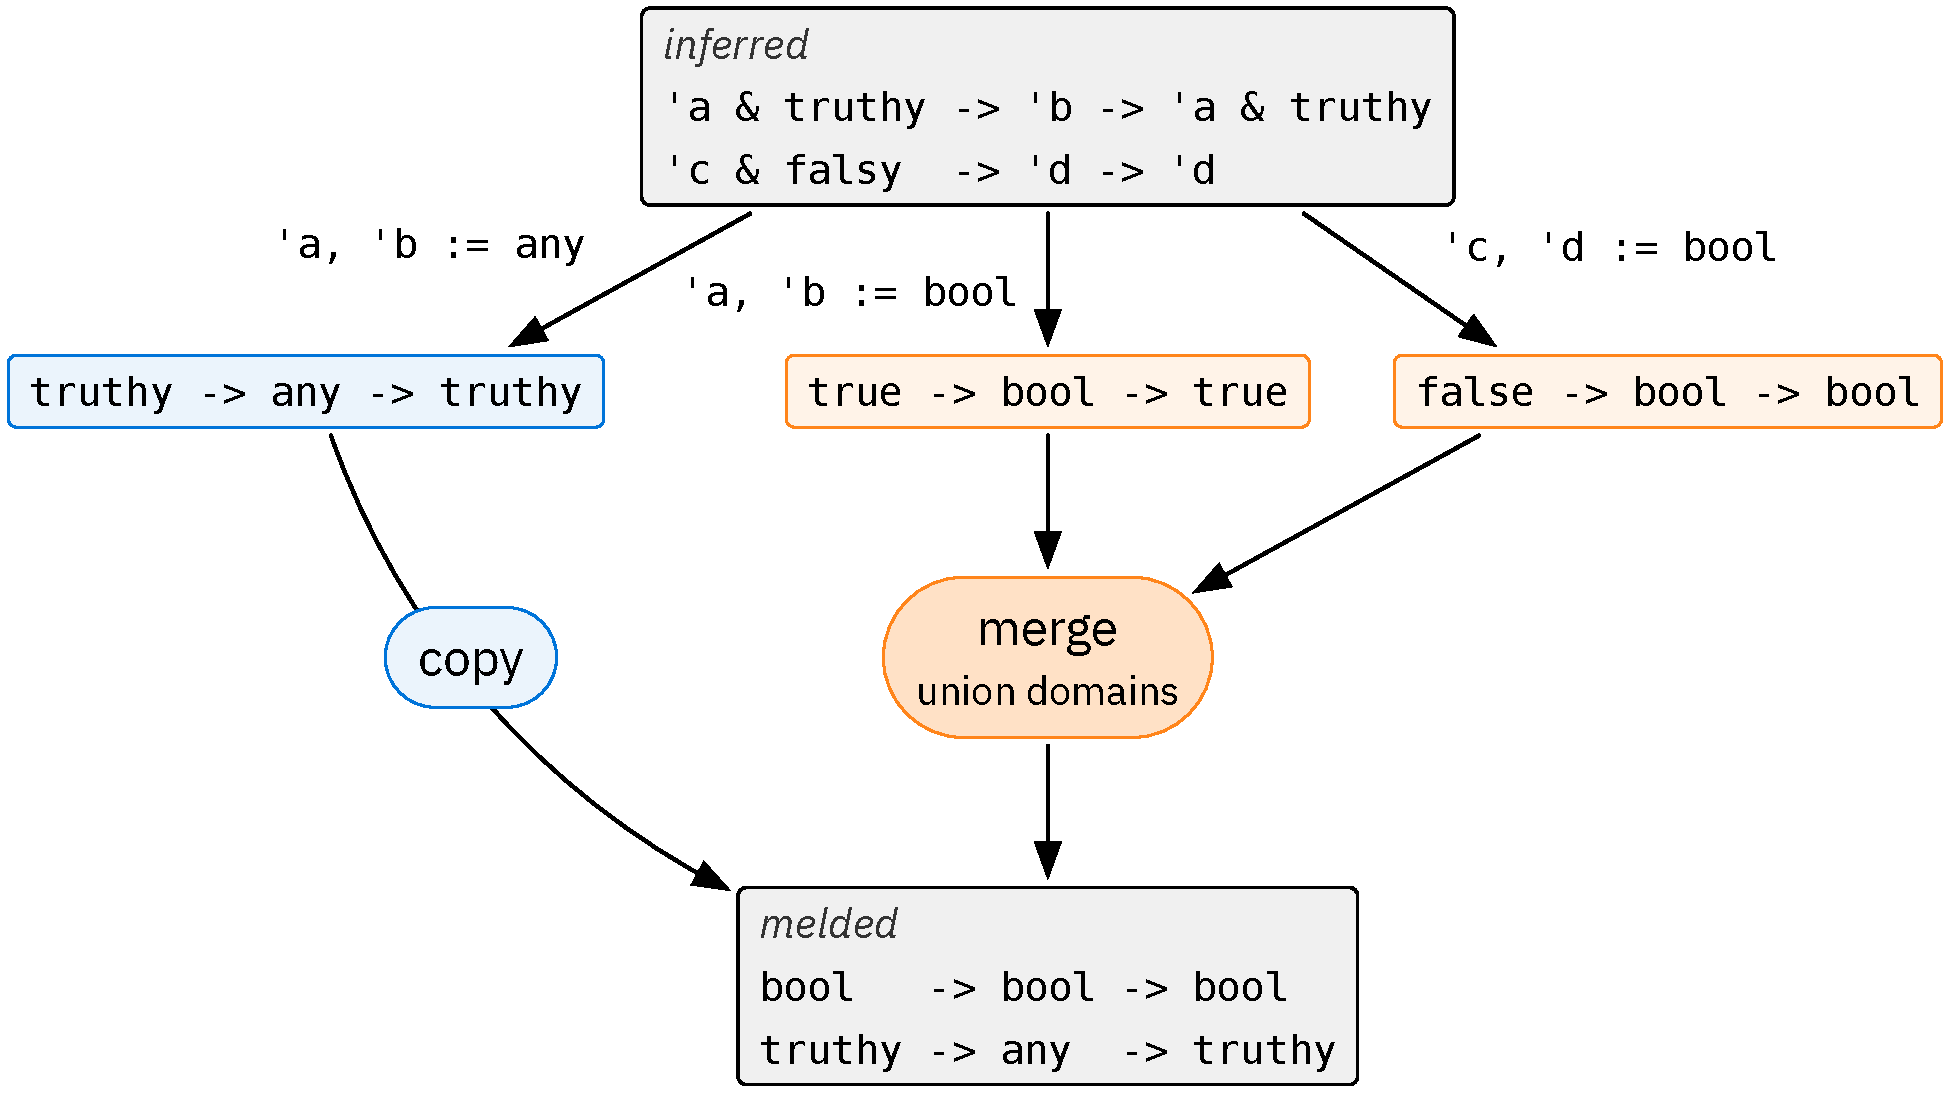
\includegraphics[width=\linewidth]{refine-diagram.pdf}
  \caption{Instantiate and merge operations reshaping the inferred
    signature of \ttt{logical\_or}.}
  \Description{Diagram showing the inferred signature of logical\_or
    being instantiated and merged into simpler signatures.}
  \label{fig:refine}
\end{figure}

From the inferred type above, applying the operations yields
simpler and less precise signatures:

\begin{lstlisting}[language=MLsem]
val logical_or : bool -> bool -> bool
val logical_or : truthy -> any -> truthy
\end{lstlisting}

The first is the familiar boolean reading and the second keeps the
``returns its first argument when truthy'' behaviour but drops the
polymorphism.  The toolkit makes the choice between them explicit.

\begin{figure}
  \centering
  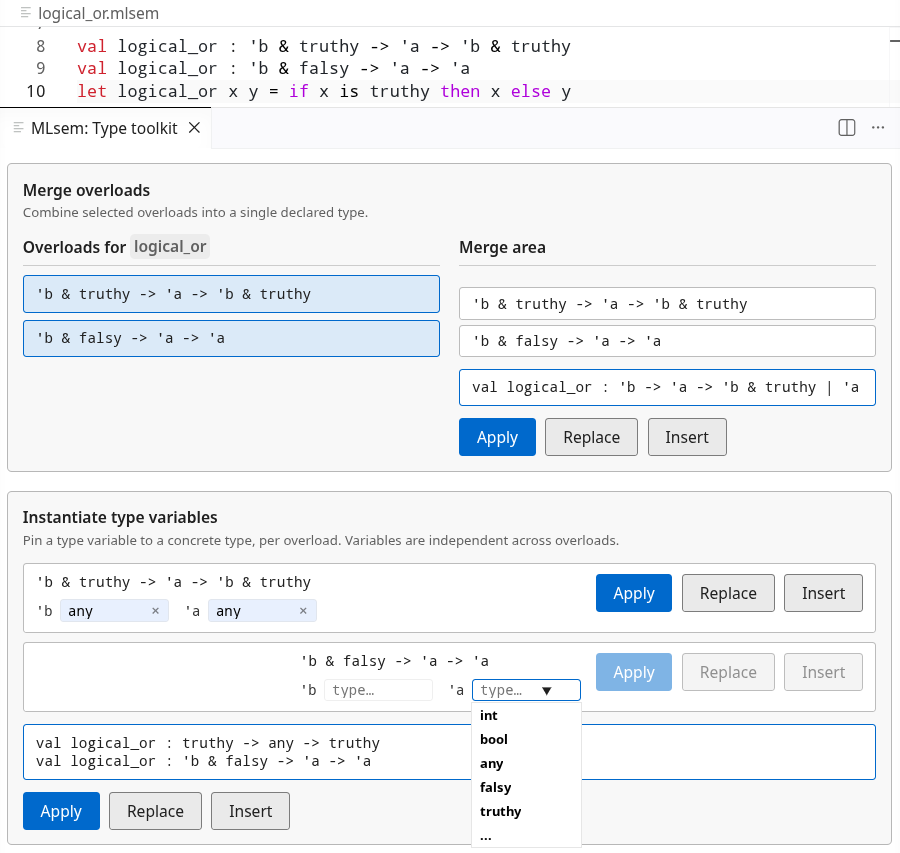
\includegraphics[width=\linewidth]{toolkit.png}
  \caption{The merge and instantiate panels of the VS~Code extension.}
  \Description{Screenshot of the VS Code extension showing the merge
    overloads and instantiate type variables panels.}
  \label{fig:toolkit}
\end{figure}

The toolkit provides these operations using an integrated
interface as a VS~Code extension, as depicted in
Figure~\ref{fig:toolkit}.
It is available at \url{https://github.com/asmarcz/MLsem-vscode}.

\section{Future direction: moving to R}

More operations are planned, notably \emph{domain decomposition}
and \emph{branch specialization}.

Our target is the R language.  It is deeply dynamic ---
coercions, promises, and multiple dispatch
mechanisms --- so~precise inference produces unreadable types, while
readable types require judgement calls that only the programmer can
make.  The toolkit eases this
trade-off: inference supplies the precise starting point, the user
steers the simplification.

Several directions remain open: LLM-assisted trade-off search guided
by user-provided success criteria, operations for language-specific
features such as builtin dispatch, and extending the approach to
modules and objects. Runtime feedback could also guide the shape of the types.

\begin{acks}
This work is supported by the Czech Ministry of Education, Youth and Sports under program ERC-CZ, grant agreement LL2325,
        as well as by the Czech Science Foundation Grant No.~23-07580X.
\end{acks}

\bibliographystyle{ACM-Reference-Format}
\bibliography{refs}

\end{document}
